\chapter{Introduction}

Complex systems are evertwhere around us:
\begin{itemize}
    \item Traffic systems;
    \item Disease spereading (e.g. COVID);
    \item dynamics of social networks;
    \item Natural ecosystems (take inspiration from nature evolution);
    \item Software systems.
\end{itemize}

\begin{minipage}{0.45\textwidth}
    \centering 
    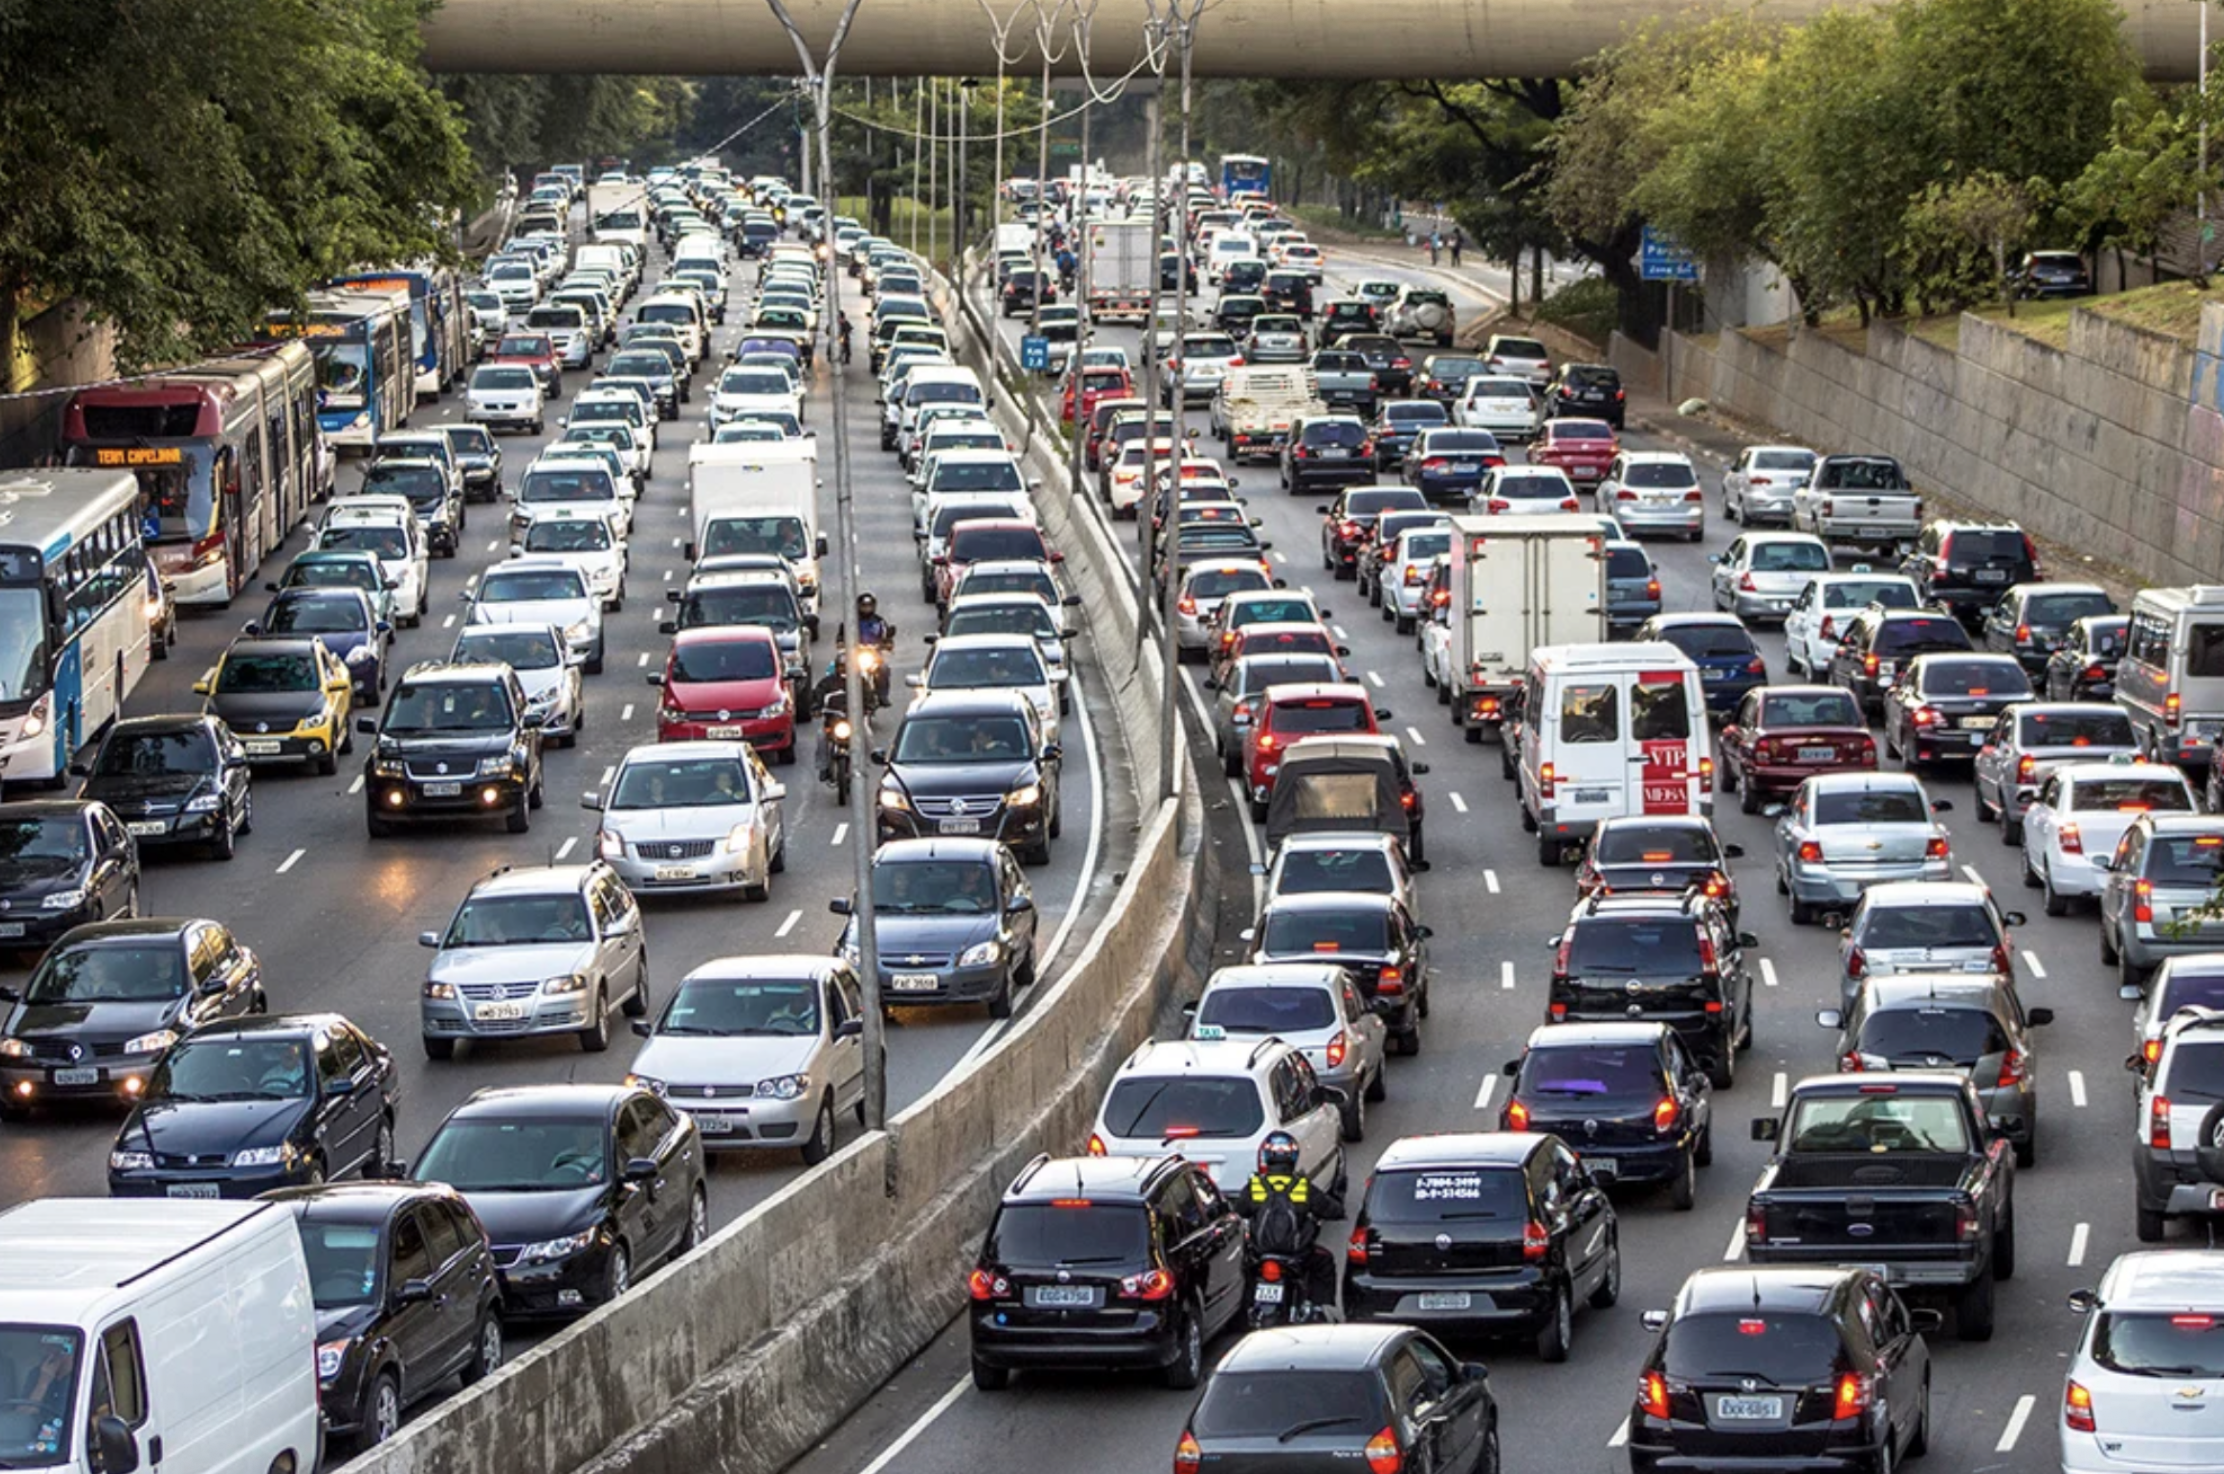
\includegraphics[width=\textwidth]{assets/ch1/1.png}
    \captionof{figure}{Traffic.}
    \label{fig:traffic} 
\end{minipage}
\hfill
\begin{minipage}{0.45\textwidth}
    \centering
    \includegraphics[width=\textwidth]{assets/ch1/2.png}
    \captionof{figure}{Social networks.}
    \label{fig:social}
\end{minipage}

\begin{definitionblock}[Complex System]
    A \textbf{Complex System} is composed by many components interactinv in a non-trivial way. A specific case could be: "How can we analyze traffic in our city?"
    \begin{itemize}
        \item Traditional analytical methods;
        \item Simulation-based methods;
        \item Mathematical optimization;
        \item Directed graphs;
        \item ... 
    \end{itemize}
\end{definitionblock}

There are several approaches to the problem. We need to simplify the model first, otherwise there would be so many variables to consider that it would be impossible to analyze them all together. Then, we can focus on different aspects of the problem, using different models for each to capture the relevant dynamics. Finally, we can integrate these models to get a comprehensive understanding of the system as a whole.
At the beginning it is a sort of \textit{black-box}, in the sense that we do not know how the system works internally, but we can observe its inputs and outputs. The goal is to understand the internal mechanisms that drive the system's behavior.

\begin{definitionblock}[Black-box models]
    \textbf{Black box} models focus on modeling the relationships between inputs and outputs on a system, without explicitly considering the internal processes that generate those outputs from the inputs.
    They are widely used today and are based purely on observed input/output data from the system, without knowledge of the internal mechanism. See for example Neural Networks, statistical models or machine learning algorithms.
    They lack \textbf{explainability}. 
\end{definitionblock}

We need something complex enough to capture the dynamics of the system, but simple enough to be tractable.

\textbf{Agents} are another way to model complex systems. Intelligent agents excel at modeling individual behavior and the emergence of global phenomena:
\begin{itemize}
    \item Individual behavior is simple;
    \item Interactions are complex;
    \item Macroscopic behavior emerges from microscopic interactions.
\end{itemize}

\begin{figure}[H]
    \centering
    \includegraphics[width=0.6\textwidth]{assets/ch1/3.png}
    \caption{The world with agents}
    \label{fig:agents_world}
\end{figure}

But how can we model a problem with agents? In the case of traffic, we can model each vehicle as an agent with individual behavior, represent traffic signals and lights as agents interacting with vehicles, incorporate pedestrians agents with their own behaviors and model the road environment as a graph of interconnected agents representing intersections and road segments.

Interactions emerge from local agent behavior and each agent models an individual component with autonomy. 

\begin{tipsblock}
    This is useful for simulation and comparing with real world scenarios.
\end{tipsblock}

At the end we can simulate different scenarios by modifying parameters, or analyze the emergence of traffic jams from individual behaviors, explore strategies to optimize circulation or calibrate and validate the model with real city data.

\textbf{Intelligent Agent Systems} are systems composed by multiple interacting agents, in which intelligence emerges from interactions among agents and between agents and the environment. Such intelligence encompasses learning, reasoning, social interaction and other capabilities that are human-like. 

Examples of intelligent agents can be found in various domains:
\begin{itemize}
    \item An automated personal assistant that can make reservations, respond to emails and organize our schedule autonomously;
    \item An intelligent virtual tutor that can teach us new topics and adapt to our learning style;
    \item Autonomous cars or delivery drones.
\end{itemize}

\begin{observationblock}[Agents today]
    Recent advancements include interactions with the user while maintaining \textbf{context}:
    \begin{itemize}
        \item \textbf{Memory Integration}: persistent memory to maintain long-term context;
        \item \textbf{Multi-modal Capabilities}: Understanding text and images;
        \item \textbf{Execution of actions}: interacting with external tools and APIs.
    \end{itemize}
    Advancements in cooperative AI has been also made, enabling agents to collaborate at solving problems in real-world applications such as in healthcare, logistics and resource management. 
    Moreover, cognitive architectures are being developed to endow agents with human-like reasoning and decision-making capabilities, enhancing their ability to operate in complex and dynamic environments.
    \begin{itemize}
        \item \textbf{SOAR Cognitive Architecture}
        \item \textbf{ACT-R Cognitive Architecture}
        \item \textbf{Transformers}
    \end{itemize}
\end{observationblock}

